\documentclass[11pt]{article}

\hoffset        2mm 
\voffset        -15mm
\oddsidemargin  0mm
\topmargin      0.30in
\textwidth      6.25in
\textheight     9in

\usepackage[parfill]{parskip}
\usepackage{graphicx}
\usepackage{amsmath}
%\usepackage{mathtools}
\usepackage{booktabs}
\usepackage{enumerate}
\usepackage{listings}
\usepackage{float}
\usepackage{bigints}
\usepackage{caption}
\usepackage{subcaption}
\usepackage{afterpage}

\begin{document}


\begin{center}
{\Large PhD Dissertation Proposal}\\[6mm]
{\Large DFEM $S_N$ Transport Calculations on Unstructured Polytope Meshes}\\[8mm]
{Michael W. Hackemack} \\[2mm]
{\em \small Department of Nuclear Engineering, Texas A\&M University, College Station, TX 77843, USA} \\[1mm]
{\em mike\_hack@tamu.edu} \\[6mm]
\end{center}

\noindent\rule{6.25in}{0.4pt}

{\Large \bf Abstract}
\vspace{2mm}

The discontinuous finite element method (DFEM) has been widely used to solve the radiation transport equation using the discrete ordinates ($S_N$) approximation. The bulk of this work has been on simplical and canonical mesh types (triangles, tetrahedron, quadrilaterals, and hexahedron). Only more recently has work begun to emerge in the community to analyze transport solutions on polytope meshes (polygons and polyhedron). The ultimate goal of this dissertation is to extend our applicable knowledge in solving the DFEM transport equation on polytopes by focusing on higher order FEM trial spaces as well as acceleration methodologies on massively parallel computer architectures.

Progress towards this goal has been made in different phases. First, it has been shown that the symmetric interior penalty (SIP) method can function as a discontinuous formulation of the diffusion equation on arbitrary polyhedral grids. Next, transport acceleration by diffusion synthetic acceleration (DSA) using the modified interior penalty (MIP) method was implemented in the Parallel Deterministic Transport (PDT) code at Texas A\&M University. Finally, a general, object-oriented, FEM, MATLAB program has been written to solve the transport and diffusion equations on arbitrary polytope meshes, with different basis function sets of different trial space orders.

To complete this project, scaling studies of MIP DSA on both structured and unstructured polygonal/polyhedral grids needs to be performed. We will collect both estimates of the numerical spectral radius (NSR) and timing statistics to analyze the method's performance. We will complete the dissertation work by analyzing higher order (specifically quadratic) FEM trial spaces on 2D polygonal grids.

\noindent\rule{6.25in}{0.4pt}

%%%%%%%%%%%%%%%%%%%%%%%%%%%%%%%%%%%%%%%%%%%%%%%%%%%%%%%%%%%%%%%%%%%%%%
%%%%%%%%%%%%%%%%%%%%%%%%%%%%%%%%%%%%%%%%%%%%%%%%%%%%%%%%%%%%%%%%%%%%%%
\section{Introduction}
\label{sec::intro}

The solution of the {\em First-Order Boltzmann Transport Equation}, which we will simply call the transport equation for brevity, has myriad uses across multiple fields \cite{duderstadt1979transport,duderstadt1976nuclear}. From medicine, power, oil exploration, food and product irradiation, astrophysics, and weapons technologies, finding solutions to the transport equation is becoming more ubiquitous across different industries. Over the years, various computer codes have been developed to solve the transport equations via different solution techniques \cite{hill1975onetran,reed1973triplet,seed1978trident,mordant1981some,ref::geant4,ref::MCNP,ref::DANTSYS,ref::TORT,ref::PENTRAN,ref::TRITON,ref::NEWT}. In no way do we claim that this is an exhaustive list of transport code examples.

Currently, the largest radiation transport problems are running on machines operating at the petaflop level ($10^{15}$ floating point operations per second). In more recent years, there has been a push by the United States Department of Energy (DoE) to push the computational power devoted to radiation transport problems to the exascale level \cite{bergman2008exascale}. Many areas of research are still required to see this exascale computing goal come to fruition. This includes, but is not limited to, computer architectures, numerical methods, mesh generation, and more. One area of development that will enhance the exascale project is further methods development on polytope meshes (arbitrary polygons and polyhedra). Some of the main benefits for using arbitrary polygonal/polyhedral meshes are the following:

\vspace{4mm}
\begin{enumerate}
	\item Polytope mesh cells are now being employed in other physics communities - most notably computational fluid dynamics (CFD)\cite{ref::star_CCM};
	\item They can allow for transition elements between different portions of the domain (e.g., tetrahedral elements bordering hexahedral elements at the border of the boundary layer);
	\item They are believed to reduce the number of unknowns to solve with equivalent accuracy;
	\item They can reduce cell/face counts which can reduce algorithm wallclock times depending on the solution method;
	\item They can easily be split along cut planes - allowing the mesh to be partitioned into regular or irregular divisions as well as be generated by simplical meshing techniques across processor sets in parallel;
	\item Hanging nodes from non-conforming meshes, like those that naturally arise from locally refined/adapted meshes, are no longer necessary. 
\end{enumerate}
\vspace{4mm}

Benefits 3-6 can directly impact the DoE's desire to extend radiation transport calculations to the exascale level. Benefits 3 and 4 directly impact large-scale transport simulations because they can help to reduce algorithm setup and execution times. For programs that have to do a lot of inner iterations looping through cells and interior faces, reducing these counts can have significant benefit. Benefits 5 and 6 can also play an appreciable role in large-scale transport simulations. Polytope elements allow for the domain to be meshed in parallel with simplical mesh generators \cite{shewchuk1996triangle,shewchuk2002delaunay,si2006quality,geuzaine2009gmsh} and then stitched together at processor interfaces. This procedure will yield degenerate polygons (in 2D) and degenerate polyhedra (in 3D). These degenerate polytopes would normally require the use of hanging nodes, like those that naturally arise in adaptive mesh refinement (AMR) \cite{plewa2005adaptive,berger1984adaptive,oden2001goal,vsolin2004goal}. However, if one uses polygonal finite element spaces, then the coding complexity of dealing with hanging nodes is removed. An example of these degenerate polytope elements is given in Figure \ref{fig::LRN} with a 2D AMR example.

\begin{figure}[!ht]
\vspace{2mm}
\centering
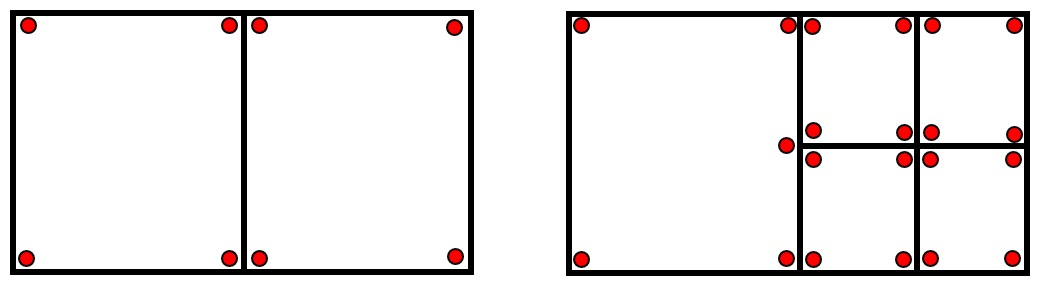
\includegraphics[width=0.80\textwidth]{figures/locally_refined_nodes.png}
\caption{Example of a pair of quadrilateral cells (left) before and (right) after refinement. The unrefined spatial cell on the left becomes a degenerate (weakly convex) pentagon after refinement of the right cell.}
\vspace{2mm}
\label{fig::LRN}
\end{figure}

%%%%%%%%%%%%%%%%%%%%%%%%%%%%%%%%%%%%%%%%%%%%%%%%%%%%%%%%%%%%%%%%%%%%%%
%%%%%%%%%%%%%%%%%%%%%%%%%%%%%%%%%%%%%%%%%%%%%%%%%%%%%%%%%%%%%%%%%%%%%%
\section{Objective}
\label{sec::obj}

The objective of this research is to help advance the state of the art in solving the transport equation via discrete ordinates ($S_N$) using the linear discontinuous finite element method (LDFEM). Specifically, we will focus our research on the use of polygonal/polyhedral finite element spaces due to their myriad benefits as outlined in Section \ref{sec::intro}. We will concentrate our work on two main topical areas: 1) higher order (2nd) transport solutions on polygons using quadratic serendipity basis functions and 2) extensions of transport acceleration using MIP DSA.

MATLAB will be used for all the necessary prototype work regarding analysis of the FEM transport solutions using higher order basis function sets on polytopes. This analysis includes the use and limitations of these higher order trial spaces. We especially will analyze the geometric limitations that must be placed on the mesh to ensure accurate solutions.

Finally, the PDT code will be used to analyze transport acceleration using MIP DSA on polytope meshes. Work will consist of three main areas. First, comparative analysis will be performed between numerical and analytical results from fourier analysis on canonical shapes. Second, scaling studies will be done to analyze how MIP DSA acceleration will perform at large core counts $(O(10^5) - O(10^6))$ for both neutronics and TRT problems. This will consist of both structured and unstructured mesh partitions. Finally, comparative analysis will be performed with MIP for TRT problems with a DSA method consisting of a continuous finite element (CFEM) trial space with a discontinuous update of the absorption rate density (ARD).

%%%%%%%%%%%%%%%%%%%%%%%%%%%%%%%%%%%%%%%%%%%%%%%%%%%%%%%%%%%%%%%%%%%%%%
%%%%%%%%%%%%%%%%%%%%%%%%%%%%%%%%%%%%%%%%%%%%%%%%%%%%%%%%%%%%%%%%%%%%%%
\section{Present Status of the Question}
\label{sec::PS}

For years, the discontinuous finite element method (DFEM) has been used to solve the discrete ordinates transport equation for both neutronics and thermal radiative transfer (TRT) problems \cite{hill1975onetran,reed1973triplet,larsen1982finite,larsen1987asymptotic,larsen1989asymptotic,adams2001dfem}. These efforts have primarily focused on using linear trial spaces which leads to the linear discontinuous finite element (LDFEM) form of the transport equation. Some research has also gone into using higher order DFEM trial spaces \cite{walters1986relation,hennart1995generalizedI,hennart1995generalizedII,wang2009convergence,wang2009adaptive,warsa1999p,maginot2013characterization,maginot2015lumping}. 

In more recent years, a general push has been occurring to obtain higher fidelity transport solutions on larger and larger computer architectures. However, due to the large dimensional space of the transport equation (energy and angle), efficiently inverting the full transport matrix can be prohibitive. Instead, a matrix-free method would minimize memory requirements and allow the majority of the computational burden to lie on CPU/GPU operations, which coincides with the findings on the DoE exascale analysis \cite{bergman2008exascale}. A common matrix-free methodology to solve the discretized transport equation with upwinding is called the transport sweep \cite{ref::adams_larsen_iter_methods}. Transport sweeps also hold the desirable property that iteration counts do not grow with mesh refinement.

Because parallel execution of the transport sweep leaves some tasks unable to begin until previous levels of the graph finished, a common perception arose that parallel sweeps would not efficiently scale past a few thousand processes \cite{evans2010denovo,zerr2011solution}. At the time, various partitioning and scheduling algorithms had been developed including: data driven algorithms \cite{dorr1996concurrent,brown1999performing,brown1999performing}, the Compton-Clouse (CC) algorithm \cite{compton2005tiling}, and the popular Koch-Baker-Alcouffe (KBA) algorithm \cite{ref::KBA,baker1998s}. While KBA yielded better performance than previously realized, all these algorithm devised non-optimal parallel scheduling when they construct their task graphs. Recently, work has gone into developing efficient and provably optimal sweeping strategies that will allow sweep scaling out to $O(10^6)$ processes and beyond \cite{ref::eff_sweeps,adams2013provably}. All of this work was performed with the PDT code built on top of the Standard Template Adaptive Parallel Library (STAPL) \cite{buss2010stapl,tanase2011stapl,buss2011stapl,fidel2013stapl}.

To date, the bulk of the parallel sweep scheduling algorithms have been analyzed on regular, cartesian grids. However, some research has gone into obtaining transport solutions on unstructured meshes. The TRIPLET \cite{reed1973triplet}, TRIDENT \cite{seed1978trident}, and ZEPHYR \cite{mordant1981some} codes solved the DFEM transport problem on unstructured 2D triangular meshes. Wareing et. al. then devised efficient DFEM transport solutions on unstructured 3D grids \cite{wareing2001discontinuous}. This work was then extended to unstructured parallel sweep scheduling \cite{pautz2002algorithm,zeyao2004parallel,mathis2004performance}. Effectively devising efficient parallel sweeping strategies for unstructured meshes remains an open topic of research.

The ability to efficiently invert the transport (streaming and collision) operator does not necessarily mean that transport solutions can be easily obtained. In general, radiation transport solutions are obtained iteratively. The simplest and widely-used method is a fixed-point scheme ({\em i.e.} richardson iteration) ubiquitously called source iteration (SI) in the transport community. Unfortunately, the iteration process of SI can converge arbitrarily slowly if the problem is optically thick \cite{ref::adams_larsen_iter_methods}. This corresponds to long mean free paths for neutronics problems. This also corresponds to time steps and material heat capacities tending to infinity and zero, respectively, for TRT problems.

For these problem regimes in which solution is prohibitively slow, additional steps should be taken to speed up, or accelerate, solution convergence \cite{ref::adams_larsen_iter_methods}. The most used methods to assist in solution convergence are often called synthetic acceleration techniques. These techniques were first introduced by Kopp  \cite{kopp1963synthetic} and Lebedev \cite{lebedevI,lebedevII,lebedevIII,lebedevIV,lebedevV,lebedevVI,lebedevVII} in the 1960's. From Kopp's and Lebedev's work, Gelbard and Hageman then introduced two synthetic acceleration options for the low-order operator: diffusion and $S_2$ \cite{gelbard1969synthetic}. Their diffusion preconditioning led to efficient convergence properties on fine spatial meshes. Reed then showed that Gelbard and Hageman's diffusion preconditioning would yield a diverging system for coarse meshes \cite{reed1971effectiveness}. At this point in time, no one knew if an unconditionally efficient acceleration method could be derived.

Then in 1976, Alcouffe proposed a remedy to Gelbard and Reed that he called diffusion synthetic acceleration (DSA) \cite{alcouffe1976stable,alcouffe1977DSA,alcouffe1977diffusion}. He showed that if you derived the diffusion operator consistently with the discretized transport operator, then SI could be accelerated with DSA in an efficient and robust manner. Larsen and McCoy then demonstrated that unconditional stability required that consistency be maintained in both spatial and angular discretization in their four-step procedure \cite{larsen1982unconditionally_I,larsen1982unconditionally_II}. However, Adams and Martin then showed that partially-consistent diffusion discretizations could effectively accelerate DFEM discretizations of the neutron transport equation \cite{ref::dsa_DFEM_adams_martin}. Their modified-four-step procedure (M4S), based on Larsen and McCoy's work, was shown to be unconditionally stable for regular geometries, but divergent for unstructured multi-dimensional meshes \cite{warsa2002fully}. In more recent years, alternate discretizations for the diffusion operator have been applied to unstructured multi-dimensional grids. These include the partially consistent Wareing-Larsen-Adams (WLA) DSA \cite{ref::WLA_DSA}, the fully consistent DSA (FCDSA) \cite{warsa2002fully}, and the partially consistent MIP DSA \cite{ref::DSA_wang_ragusa,wang2009adaptive,turcksin2014discontinuous}.

Most recently, the partially consistent MIP DSA method has been shown to be an unconditionally stable acceleration method for the 2D DFEM transport equation on unstructured meshes. Wang showed that it acted as an effective preconditioner for higher-order DFEM discretizations on triangles \cite{ref::DSA_wang_ragusa,wang2009adaptive}. Turcksin and Ragusa then extended the work to arbitrary polygonal meshes \cite{turcksin2014discontinuous}. The MIP diffusion operator is symmetric positive definite (SPD) and was shown to be efficiently invertible with preconditioned conjugate gradient (PCG) and advanced preconditioners such as algebraic multi-grid (AMG) \cite{turcksin2014discontinuous}.

%%%%%%%%%%%%%%%%%%%%%%%%%%%%%%%%%%%%%%%%%%%%%%%%%%%%%%%%%%%%%%%%%%%%%%
%%%%%%%%%%%%%%%%%%%%%%%%%%%%%%%%%%%%%%%%%%%%%%%%%%%%%%%%%%%%%%%%%%%%%%
\section{Current Work}
\label{sec::Current_Work}

We will now briefly report the work that has already been completed for this dissertation project. Section \ref{sec::CW_MIP} outlines the work completed towards extending MIP DSA to massively parallel architectures and Section \ref{sec::CW_quad} outlines the work completed to analyze quadratic finite element basis functions in arbitrary polygons.

%%%%%%%%%%%%%%%%%%%
\subsection{MIP DSA on Polyhedral Meshes}
\label{sec::CW_MIP}

In our efforts to enable PDT to perform DSA at large scale on polyhedral grids, we first demonstrated that the symmetric interior penalty (SIP) method \cite{ragusa2015discontinuous}, which is a generalized DFEM diffusion form, will work on arbitrary polyhedral meshes \cite{ref::SIP_3D}. In \cite{ref::SIP_3D}, we demonstrated that, with PWL basis functions, SIP can perfectly capture purely linear solution spaces, even on highly distorted concave mesh cells. Also, the proper second-order convergence rates are captured using the Method of Manufactured Solutions (MMS) \cite{salari2000code}. 

Next, we implemented transport acceleration with DSA using the MIP diffusion form into the PDT code. The diffusion matrix can be inverted with either PDT's already coded solvers or by use of HYPRE's efficient solvers and preconditioners, which has also been successfully integrated \cite{ref::hypre}. The majority of the work to date has involved using HYPRE's PCG solver with BoomerAMG preconditioning. We have confirmed the results of Turcksin and Ragusa that PCG using AMG preconditioning is far superior than simple Jacobi or SSOR preconditioning for inverting the MIP system matrix \cite{turcksin2014discontinuous}.

Appropriate transport acceleration has been verified in 2D and 3D even on distorted (non-orthogonal) cells. For 3D hexahedral cells, we have verified that our implementation in PDT captures the appropriate spectral radius as theorized by fourier analysis. Some of these numerical spectral radii results from PDT as well as the theoretical fourier analysis results are presented in Figure \ref{fig::fourier_NSR}. In Figure \ref{fig::fourier_NSR}, we provide results for two different runsets where the only parameter changed is the constant  in the penalty coefficient of the MIP form. It is noted that the divergence of the numerical and fourier results in the optically thin regime arises from inconsistency in the boundary formulation as previously presented \cite{wang2009adaptive,ref::DSA_wang_ragusa}. One can see in Figure \ref{fig::fourier_NSR} that the effectiveness of DSA with MIP can vary by how much the inter-cell jump is penalized. This is a known generalized behavior of interior penalty diffusion forms \cite{arnold2002unified}. Wang also demonstrated that this behavior arises for MIP DSA on triangles \cite{wang2009adaptive}. We have also demonstrated that the dimensionality, cell type, and cell distortion determine how much penalizing should be applied, but these results are not presented for brevity.



\begin{figure}[!ht]
\centering
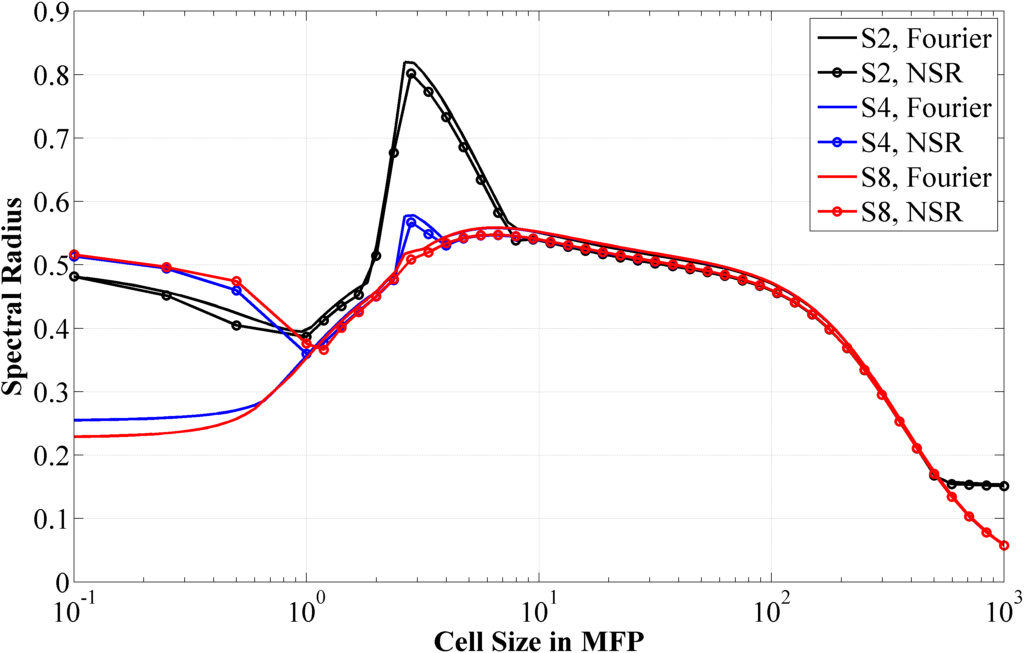
\includegraphics[width=0.95\textwidth]{figures/SI_MIP_hex_C=1_LS2,4,8_F&NSR_PDT.png}

\vspace{8mm}

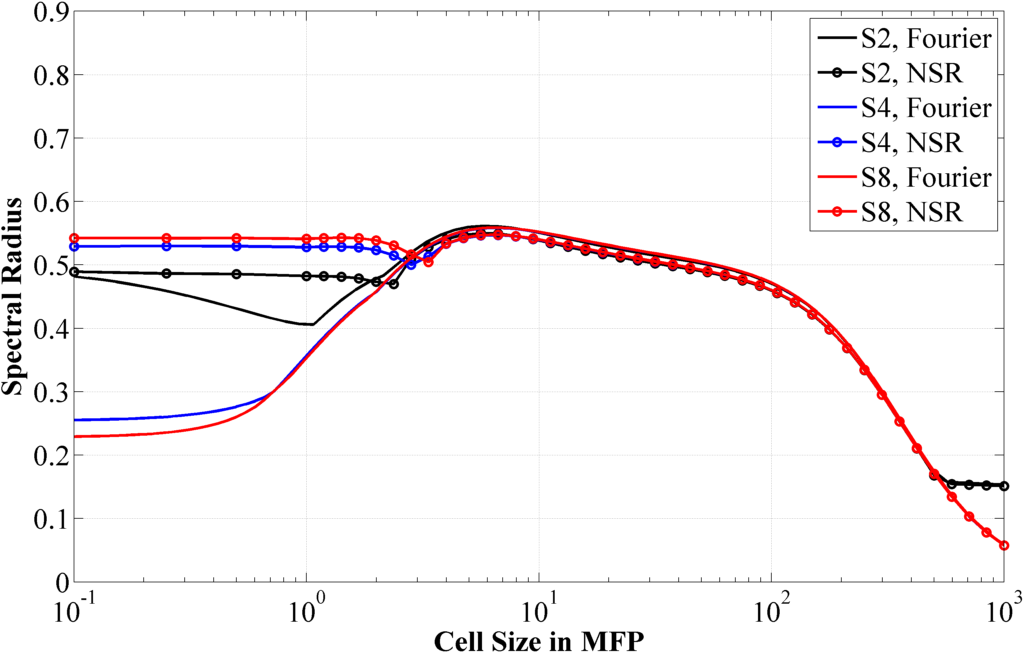
\includegraphics[width=0.95\textwidth]{figures/SI_MIP_hex_C=4_LS2,4,8_F&NSR_PDT.png}
\caption{Fourier and PDT numerical spectra radius results on a unit cube for different quadrature levels with the MIP penalty coefficient, $C=1$ (top) and $C=4$ (bottom).}
\label{fig::fourier_NSR}
\end{figure}

%%%%%%%%%%%%%%%%%%%
\subsection{Quadratic Serendipity Finite Elements for the Transport Equation on Polygonal Meshes}
\label{sec::CW_quad}

To analyze $S_N$ transport calculations on arbitrary polygons/polyhedra with higher-order basis functions, extensive work has been performed to develop a general, object-oriented MATLAB program. Many different basis functions have been implemented, including standard $P_r$, $Q_r$, and $S_r$ basis functions on simplexes and quads/hexes. Basis functions that capture linear precision on polygons and polyhedra, including PWL \cite{ref::PWLD_stone_adams,ref::PWLD_stone_adams_unstructured,bailey2008phd,bailey2011piecewise}, Wachspress \cite{wachspress1975rational}, Mean Value \cite{floater2003mean,floater2005mean,hormann2006mean}, and Maximum Entropy \cite{sukumar2004construction,sukumar2005maximum,hormann2008maximum}, have also been implemented. Figure \ref{fig::poly_flux} shows the scalar flux solution for a simple, homogeneous, source-driven DFEM transport problem using these 4 different polygon-compatible, linear basis function sets. The advantages and limitations of each of these basis function sets have been characterized for use in radiation transport calculations (as well as in general mathematical terms by the literature). 

We have also implemented the quadratic serendipity extension of the maximum entropy basis functions \cite{sukumar2013quadratic} which uses the framework of Rand \cite{rand2014quadratic}. Quadratic interpolation precision is captured along with third order convergence for parabolic problems if appropriate quadrature sets are employed. Additional precautions must be taken so that the polygonal quadrature sets are stable and can satisfy the patch test \cite{sukumar2013quadratic,dunavant1985high,krongauz1997consistent,puso2008meshfree,duan2012second}. 

\begin{figure}
\centering
	\begin{subfigure}[b]{0.48\textwidth}
		\centering
		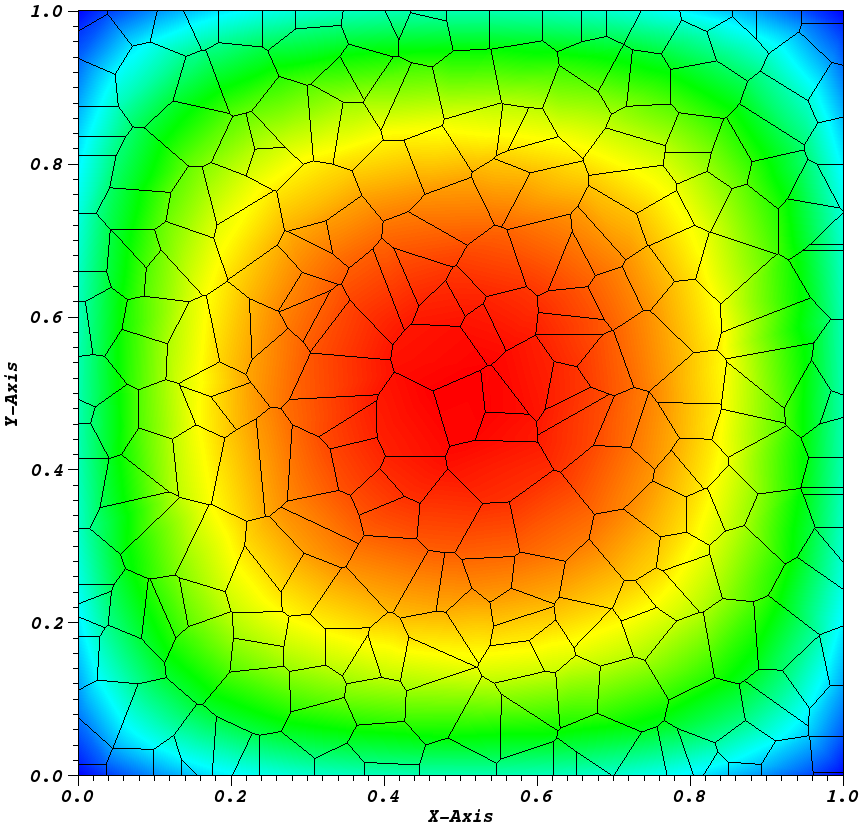
\includegraphics[width=\textwidth]{figures/poly_flux_Wachspress.png}
		\caption{}
	\end{subfigure}
	\hfill
	\begin{subfigure}[b]{0.48\textwidth}
		\centering
		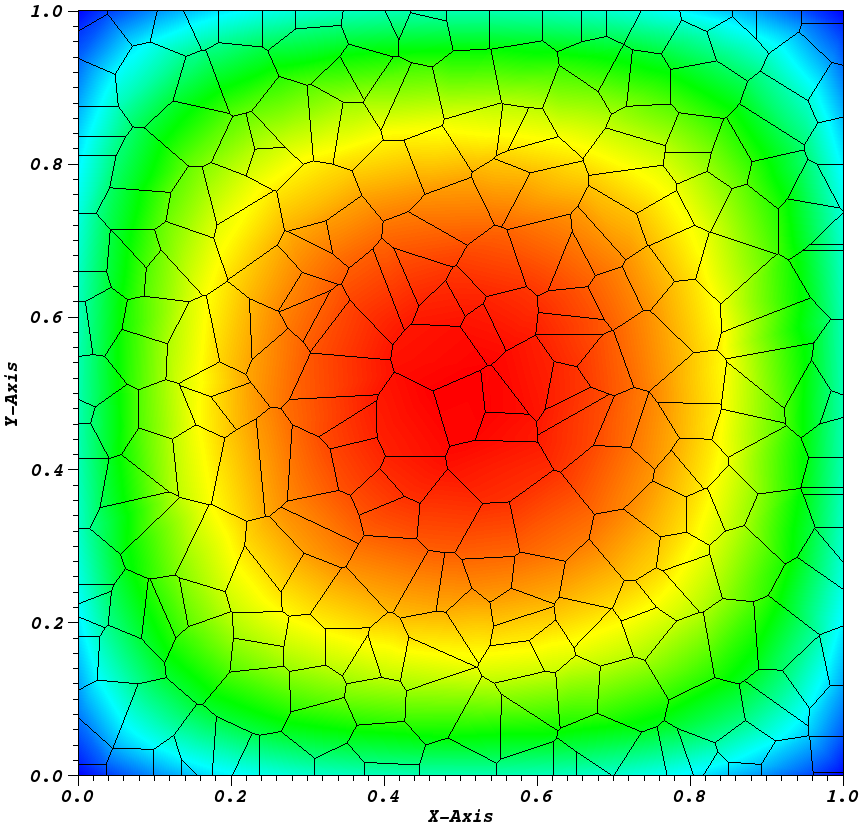
\includegraphics[width=\textwidth]{figures/poly_flux_MV.png}
		\caption{}
	\end{subfigure}
	
	\vspace{4mm}
	
	\begin{subfigure}[b]{0.48\textwidth}
		\centering
		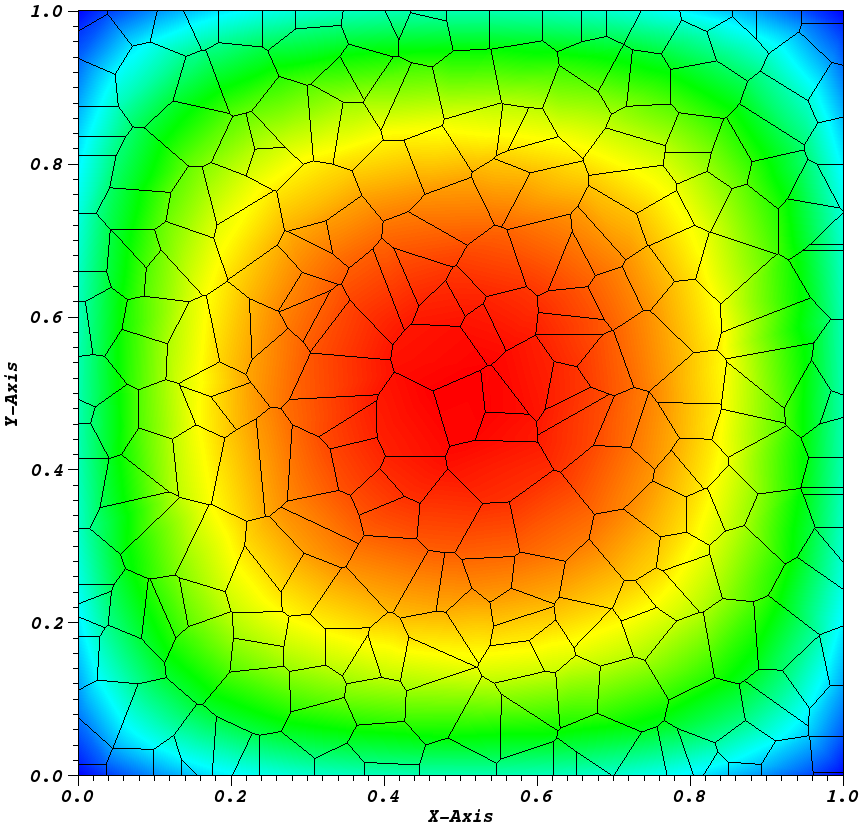
\includegraphics[width=\textwidth]{figures/poly_flux_Max_Ent.png}
		\caption{}
	\end{subfigure}
	\hfill
	\begin{subfigure}[b]{0.48\textwidth}
		\centering
		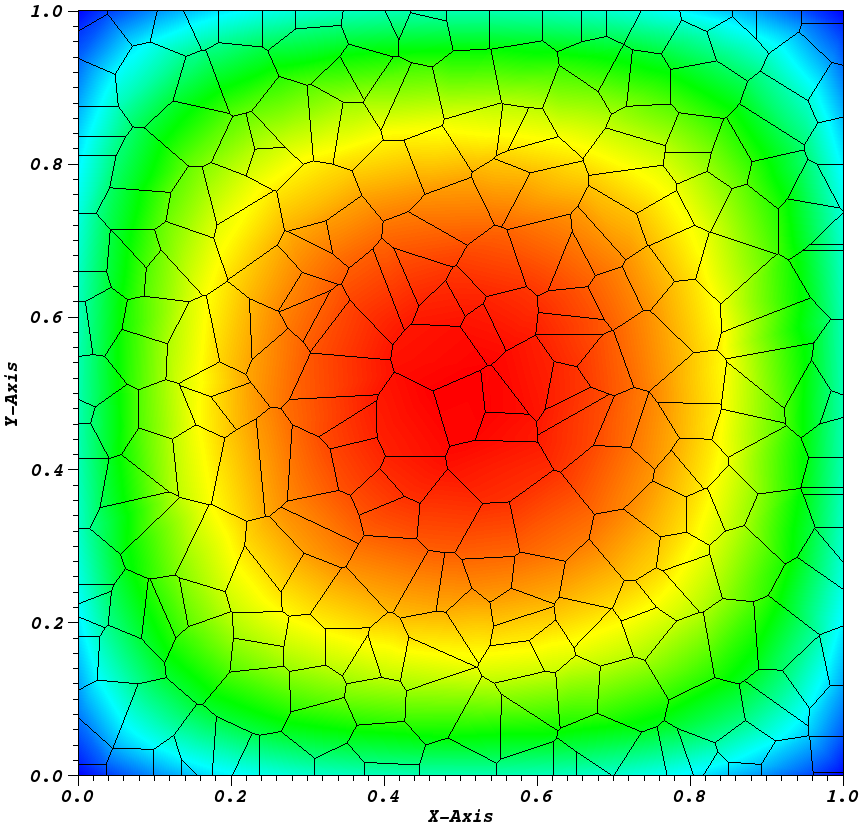
\includegraphics[width=\textwidth]{figures/poly_flux_PWL.png}
		\caption{}
	\end{subfigure}
\caption{Scalar flux solution of a simple, homogeneous, source-driven transport problem on a polygonal mesh using: (a) Wachspress, (b) Mean Value, (c) Maximum Entropy, and (d) PWL basis functions.}
\label{fig::poly_flux}
\end{figure}


%%%%%%%%%%%%%%%%%%%%%%%%%%%%%%%%%%%%%%%%%%%%%%%%%%%%%%%%%%%%%%%%%%%%%%
%%%%%%%%%%%%%%%%%%%%%%%%%%%%%%%%%%%%%%%%%%%%%%%%%%%%%%%%%%%%%%%%%%%%%%
\section{Future Work}
\label{sec::Future_Work}

Thus far, we have presented the overall objectives of the dissertation work and the work that has been completed to this point. There are still several areas of work that need to be completed. This includes work for both the MIP DSA analysis and the higher order transport analysis using quadratic serendipity finite elements.

For MIP DSA, we need to complete all scaling studies with PDT using the HYPRE software package for both neutronics and radiative transfer problems. The bulk of this work will be performed with the BGQ compute nodes on the Vulcan machine at Lawrence Livermore National Laboratory (LLNL) since we wish to test the performance capabilities of our method to at least $O(10^5)$ processor counts. We will perform scaling on both structured and unstructured meshes, including load-imbalanced cases where the transport sweep graph depth is not consistent across all processors.


For quadratic finite elements on polygons, there are two main areas left for development and analysis. First, we will use the framework of Rand to extend other linear polygonal finite elements, to a quadratic serendipity basis set \cite{rand2014quadratic}. It is possible that some of these basis sets mentioned in Section \ref{sec::CW_quad} will not be amenable to this extension because the shape functions cannot be formed into linearly-independent function sets. Second, we will use the method of Greco and Sukumar to compute the derivatives of the maximum entropy coordinates on the cell boundaries \cite{greco2013derivatives}. The derivatives of barycentric interpolation schemes are unbounded on their domain boundaries. However, with appropriate analysis, their limits are bounded. This will allow for the calculation of the Type-2 edge matrices ($\int_{e} u \vec{n} \cdot \vec{\nabla} v$) from Wang, \cite{wang2009adaptive}, which will enable us to generate all the necessary local matrices for the MIP diffusion form. We will then also perform analysis of transport acceleration using MIP DSA with quadratic serendipity basis functions on polygons.

%%%%%%%%%%%%%%%%%%%%%%%%%%%%%%%%%%%%%%%%%%%%%%%%%%%%%%%%%%%%%%%%%%%%%%
%%%%%%%%%%%%%%%%%%%%%%%%%%%%%%%%%%%%%%%%%%%%%%%%%%%%%%%%%%%%%%%%%%%%%%
\section{Expected Results and Summary}
\label{sec::ER}

We have presented the dissertation work that has been completed to date as well as the outline for all remaining work. We now quickly summarize the main topical areas of the dissertation project:

\begin{enumerate}
	\item Understand and characterize the performance of DSA using the MIP diffusion form on polyhedral grids for both neutronics and radiative transfer problems.
	\item Characterize the scaling performance of MIP DSA to high core counts $O(10^5) - O(10^6)$.
	\item Compare the effectiveness of DSA in PDT between the MIP DFEM form and a CFEM diffusion solve with discontinuous update. This will include scaling studies up to at least $O(10^5)$ processor counts.
	\item Provide a comparative analysis of the different linear basis function sets and their benefits and limitations for radiation transport problems on polygonal meshes.
	\item Extend the analysis of polygonal transport onto quadratic finite element basis sets. This will include using the work of Greco and Sukumar \cite{greco2013derivatives} to calculate the boundary gradients for these quadratic basis sets. We will then use these boundary gradients to analyze second order MIP DSA on polygons.
\end{enumerate}

%%%%%%%%%%%%%%%%%%%%%%%%%%%%%%%%%%%%%%%%%%%%%%%%%%%%%%%%%%%%%%%%%%%%%%
%%%%%%%%%%%%%%%%%%%%%%%%%%%%%%%%%%%%%%%%%%%%%%%%%%%%%%%%%%%%%%%%%%%%%%
% References
\bibliographystyle{ans}
\bibliography{references}

\end{document}


